%------------------------------
% SECTION: Sponge and Duplex Constructions 
%------------------------------
\section{Sponge Construction}

\label{sec:SpongeAndDuplex}
The sponge construction is a relatively new cryptographic primitive that has gained popularity since \Keccak won the Secure Hash Algorithm (SHA-3) competition in 2013 \cite{Bertoni2011_KeccakReference}\cite{NIST2012_SHA3_Winner}.
Essentially, it provides a way to generalize hash functions (which normally have outputs of fixed length) to functions with arbitrary length output.
This generalization allows cryptographic sponges to be used for applications other than hashing.

Sponges are based on the iteration of an underlying function $f$.
This function can either be a general \emph{transformation} or a \emph{permutation}.
The security proofs are different for transformations and permutations, and there are advantages and disadvantages for each choice of a function type \cite{Bertoni2011_SpongeFunctions}.

\begin{figure}
\centering
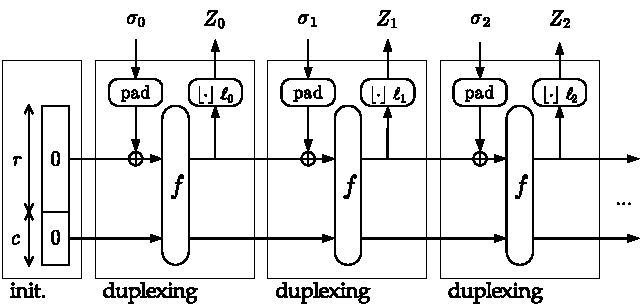
\includegraphics[width=\columnwidth]{img/Duplex.pdf}
\caption{The duplex construction $\mathbf{duplex}[f,\mathbf{pad},r]$ \cite{Bertoni2011_SpongeFunctions}}
\label{fig:Duplex}
\end{figure}

%\subsection{Sponge Parameters}
The output $Z$ of the parameterized sponge construction is given as
\begin{equation*}
\label{eq:SpongeOutput}
Z = \mathbf{sponge}[f,\mathbf{pad},r](M,\ell),
\end{equation*}
where $\mathbf{pad}$ is a padding function for the input, $r$ is the \emph{rate} of absorption, $M$ is the message (or other input) data, and $\ell$ is the desired output length.
The sponge construction re-initializes its internal state between calls to it.
It is split into two distinct phases: the \emph{absorbing} phase and the \emph{squeezing} phase.
Inputs (e.g.\ message and/or key material) are absorbed in the first phase and the output (e.g.\ a MAC or keystream) is squeezed out in the second phase.

The state of the sponge construction is split into two contiguous portions: the \emph{outer state}, which is accessible externally, and the \emph{inner state}, which is hidden.
The size of the outer state is given by the \emph{rate} $r$ and the size of the inner state is specified by the \emph{capacity} $c$.
The size of the entire state is $b = r + c$.
The speed of the construction depends on the rate, while the security depends on the capacity.

The padding function $\mathbf{pad}$ is first applied to $M$ to make it a multiple of $r$.
$M$ is then absorbed $r$ bits at a time.
More concretely, absorption is the process of XORing $r$-bit blocks into the state while interleaving with applications of the underlying sponge function $f$.
If the rate is increased then more bits are absorbed at a time and thus the construction runs faster.
However, increasing the rate means that the capacity must decrease and so there is a clear trade-off between speed and security.
Squeezing consists of concatenating $r$ bits at a time to an output bitstring $Z$ that is truncated to $\ell$ bits.
The sponge function $f$ must be called once for each $r$ bits of output after the first full block.

%------------------------------
% SECTION:Duplex Construction
%------------------------------

\section{Duplex Construction}
The duplex construction is highly related to the sponge construction.
The main differences are that the duplex construction maintains its internal state between calls rather than re-initializing it and that there no longer exists a clear separation between the absorbing and squeezing phases.
Absorbing and squeezing happen at the same time, hence ``duplexing'' \cite{Bertoni2012_Duplexing}.
The duplex mode has several applications \cite{Bertoni2010_DuplexingSlides}, with authenticated encryption being the one of interest to us.

%\subsection{Duplex Parameters}
Parameters for the duplex construction are mostly the same as for the sponge construction.
However, since the duplex construction maintains state, we build a \emph{duplex object} $D$ and make calls to it.
The function which processes inputs and produces outputs is called $\mathbf{duplexing}$:
\begin{equation*}
Z_i = D.\mathbf{duplexing}(\sigma_i,\ell_i)
\end{equation*}

Figure~\ref{fig:Duplex} shows the duplex construction.
The $i$-th input is denoted $\sigma_i$ and the $i$-th output is denoted $Z_i$, which is truncated to $\ell_i$ bits.
Inputs are absorbed and processed at the same time that outputs are squeezed.
For a duplex object it is possible to have an empty input or to not produce an output.
A \emph{blank call} is a call to $\mathbf{duplexing}$ for which no input is provided ($|\sigma_i| = 0$).
A \emph{mute call} is a call for which no output is produced ($\ell_i = 0$).

\subsection{Duplex for Authenticated Encryption}
Authenticated encryption is easily achieved using the duplex construction.
Figure~\ref{fig:DuplexAE_Expanded} shows such a use case.
First, we construct a duplex object $D$.
Then we absorb the key $K$ (or optionally $K||IV$ where $IV$ is an initialization vector) using one or more mute calls to $D.\mathbf{duplexing}$.
More than one mute call may be required if the length of the key exceeds the rate $r$.
We denote a header input to $D$ as $A = \left(A_0, A_1, \dots\right)$; these arbitrary length inputs are authenticated but not encrypted.
We denote a body input to $D$ as $B = = \left(B_0, B_1, \dots\right)$; these arbitrary length inputs are both encrypted and authenticated.
Header input blocks $A_i$ are absorbed using one or more mute calls to $D.\mathbf{duplexing}$.
Body input blocks $B_j$ are absorbed in a similar fashion and then the keystream $Z$ is XORed with $B$ to produce the ciphertext $C = \left(C_0, C_1, \dots\right)$.
The tag $T$ is produced using a blank call to $D.\mathbf{duplexing}$ after all header and body inputs have been processed.
$A'_{0}$ is the first header input block corresponding to the second header to be absorbed.

\begin{figure}
\centering
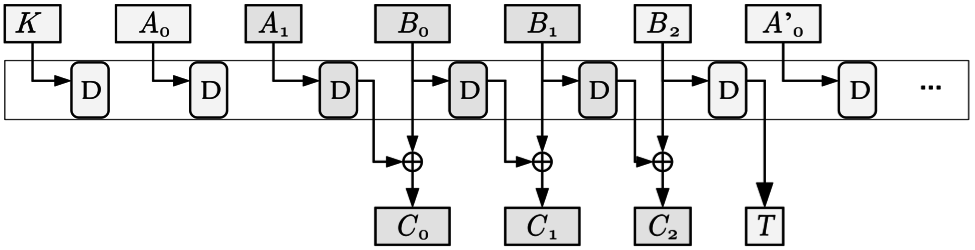
\includegraphics[width=\columnwidth]{img/DuplexAE_Expanded-BW.png}
\caption{The duplex construction as used for authenticated encryption \cite{Bertoni2010_DuplexingSlides}}
\label{fig:DuplexAE_Expanded}
\end{figure}

\begin{comment}
\begin{enumerate}
\item Easy to use
\item Single key required
\item Single-pass for encryption and authentication
\item Support for intermediate tags
\item Support for Additional Authenticated Data (AAD, or headers)
\item Secure against generic attacks
\item Ability to trade off speed and security by adjusting $r$
\end{enumerate}
\end{comment}

We note that the duplex construction may require \emph{domain separation}, a generic mechanism for eliminating output ambiguity.
For example, the simplest domain separation method consists of appending a \emph{frame bit} to the last block of every different input data type (e.g.\ key or message data).
This frame bit has the property that no two consecutive data types have the same frame bit value, meaning that one can easily identify where one data type ends and the next begins \cite{Bertoni2012_Duplexing}.

\subsection{Generic Security}
\label{sec:DuplexSecurity}
Any calls made to the duplex construction can be reduced to calls to the keyed sponge construction.
As a result, the security of the duplex construction depends only on its corresponding sponge construction.

The security of the sponge construction is based on the assumption that the underlying sponge function $f$ is secure.
That is, if $f$ is computationally indistinguishable from random then so should be the sponge construction it is instantiated within.
Consequently, cryptographers designing a system based on the sponge construction need only be concerned with designing and cryptanalyzing a secure underlying function.
The sponge construction, when used properly, is said to be secure against \emph{generic attacks} -- attacks which do not exploit any specific properties of the underlying sponge function.
We call this the \emph{generic security} of the construction \cite{Bertoni2011_SpongeFunctions}.

The generic security of keyed constructions is higher than unkeyed.
For our purposes we are interested only in the security of the keyed sponge construction where a permutation is used for $f$. 
Jovanovic et.~al\ \cite{Jovanovic2014_Beyond} proved in 2014 that the generic security level of keyed sponge constructions is lower bounded by 
\begin{equation*}
\mathrm{min}(2^{(r+c)/2}, 2^c, 2^{|K|}).
\end{equation*} 

